
\chapter{Supplementary data and figures Chapter 6}\raggedleft\textcolor{BLUEROYAL}{\LARGE{Random genetic drift sets an upper limit on mRNA splicing accuracy in metazoans}}


{\hypersetup{linkcolor=GREYDARK}\minilof\newpage}

\graphicspath{{chap6-Alternative Splicing/figures/}}

% \beginsupplement

\begin{table}[h!]
    \begin{center}                                                                       
        \includegraphics[width=\textwidth] {Table1_supp.pdf}
    \end{center}
    \caption[Description of the main features of the samples analyzed in this study]{}
    \label{table:1}
\end{table}

\begin{table}[h!]
    \begin{center}                                                                       
        \includegraphics[width=\textwidth] {Table2_supp.pdf}
    \end{center}
    \caption[Longevity and body lenth across the 53 metazoans studied]{}
    \label{table:2}
\end{table}


\begin{figure}[h]
    \begin{center}                                                                       
        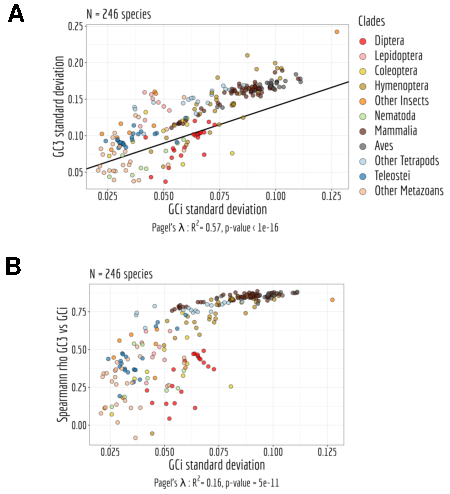
\includegraphics[width=\textwidth] {Figure1_supp.pdf}
    \end{center}                                                                       
    \caption[Transcriptome sequencing depth affects intron detection power and AS rate estimates]{\textbf{Transcriptome sequencing depth affects intron detection power and AS rate estimates.} To assess the impact of sequencing depth on AS detection, we conducted a pilot analysis with two species (\textbf{A,C}: \textit{Homo sapiens} and \textbf{B,D}: \textit{Drosophila melanogaster}) for which hundreds of RNA-seq samples are available (\hyperref[table:1]{Supplementary Tab. 1}; refer to Data10-supp.tab in the Zenodo data repository). We randomly drew 1 to 20 RNA-seq samples and, for each draw, we computed the median read coverage across BUSCO gene exons (to get a measure of transcriptome sequencing depth that is comparable across species). We also computed for each draw the average AS rate and the fraction of introns supported by at least 10 RNA-seq reads, out of all introns annotated for BUSCO genes (\nameref{sec:MaterialsMethodsAS}). We repeated this procedure 30 times. As expected, the fraction of BUSCO introns that are supported by at least 10 reads (\textit{i.e.} $\mathrm{N_s+N_a}\geq10$) increases with sequencing depth (\textbf{A,B}). More importantly, we observed that when sequencing depth is limited, the mean AS rate of BUSCO introns is very variable across draws (\textbf{C,D}). However, AS rate estimates converge when sequencing depth exceeds 200. We therefore kept for further analysis those species for which the median read coverage across exonic regions of BUSCO genes was above this threshold.}
    \label{supp_fig:AS1}
\end{figure}
    

\begin{figure}[t]   
    \begin{center}                                                                       
        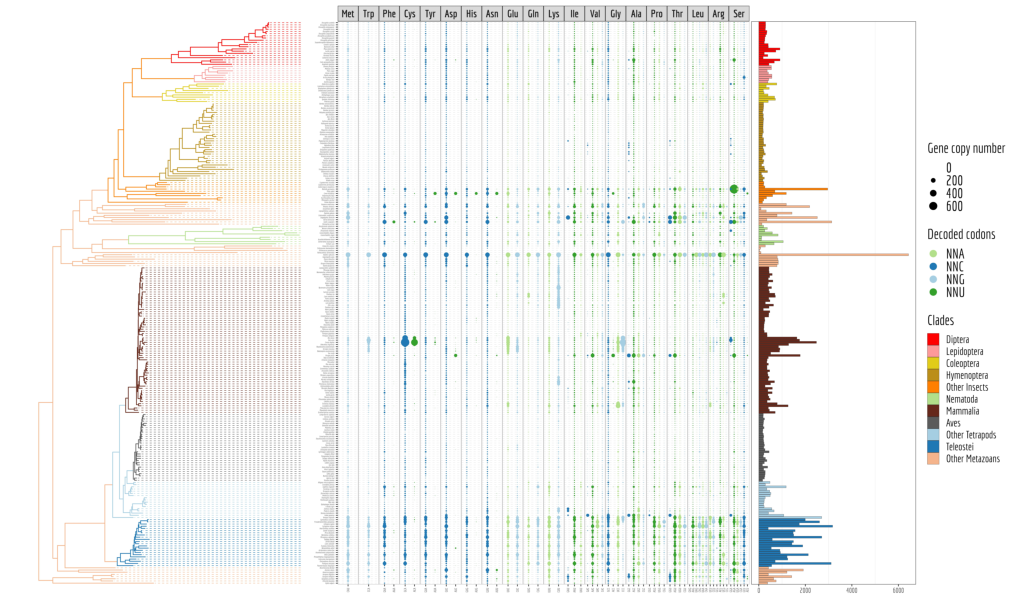
\includegraphics[width=\textwidth] {Figure2_supp.pdf}
    \end{center}                                                                       
    \caption[The power to detect AS events is positively correlated with transcriptome sequencing depth]{\textbf{The power to detect AS events is positively correlated with transcriptome sequencing depth.} Relationship between the proportion of major-isoform introns that have at least one read corresponding to splice variants (\textit{i.e.} $\mathrm{N_a}$ $>$ 0; see Fig. 2), and the median per-base read coverage computed on BUSCO gene exons, across metazoans. Each dot represents one species, colored by taxonomic clade.} 
    \label{supp_fig:AS2}
\end{figure}


\begin{figure}[t]   
    \begin{center}                                                                       
        \includegraphics[width=0.8\textwidth] {Figure3_supp.pdf}
    \end{center}                                                                       
    \caption[Relationship between AS rates and other \textit{N}$_{\text{e}}$ proxies]{\textbf{Relationship between AS rates and other \textit{N}$_{\text{e}}$ proxies.} \textbf{A,B}: Correlation between the average AS rate \textit{per} intron and the body length of each species (cm, log scale) (\textbf{A}) or the ${dN}/{dS}$ ratio on terminal branches of the phylogenetic tree (\textbf{B}). \textbf{C,D,E,F}: Relationship between the average AS rate \textit{per} intron and the body length (cm, log scale) (\textbf{C,E}) or the ${dN}/{dS}$ ratio (\textbf{D,F}). \textbf{C,D}: Low-AS major-isoform introns (\textit{i.e.} major-isoform introns that do not have any abundant SV). \textbf{E,F}: High-AS major-isoform introns (\textit{i.e.} major-isoform introns having at least one abundant SV). Only BUSCO genes were used in the analysis.}
    \label{supp_fig:AS3}
\end{figure}


\clearpage

\begin{figure}[t]   
    \begin{center}                                                                       
        \includegraphics[width=\textwidth] {Figure4_supp.pdf}
    \end{center}                                                                       
    \caption[The rate of alternative splicing correlates with life history traits in both vertebrates and insects]{
     \textbf{The rate of alternative splicing correlates with life history traits in both vertebrates and insects.} Correlation between the average AS rate per intron and longevity of each species (days, log scale) (\textbf{A,B}), body length (cm, log scale) (\textbf{B,E}), or the dN/dS ratio on terminal branches of the phylogenetic tree (\textbf{C,F}). In vertebrates (\textbf{A,B,C}) and insects 
 \textbf{C,D,E}). Only the BUSCO genes were included in the analysis.}
    \label{supp_fig:AS4}
\end{figure}


\begin{figure}[t]   
    \begin{center}                                                                       
        \includegraphics {Figure5_supp.pdf}
    \end{center}                                                                       
    \caption[The variation in AS rates between species is not explained by organ differences]{\textbf{The variation in AS rates between species is not explained by organ differences.} Variation in average AS rate across seven organs (brain, cerebellum, heart, liver, kidney, testis, and ovary) among seven vertebrate species (RNA-seq data from~\citet{cardoso-moreira_gene_2019}) and across three organs (ovary, testis, and head) for one insect (\textit{Dendroctonus ponderosae}, Coleoptera). AS rates were computed for the major-isoform introns from BUSCO genes (\nameref{sec:MaterialsMethodsAS}).} 
    \label{supp_fig:AS5}
\end{figure}


\begin{figure}[t]   
    \begin{center}                                                                       
        \includegraphics {Figure6_supp.pdf}
    \end{center}
    \caption[SNP density in human splice signals, for dinucleotides affected by CpG hypermutability]{\textbf{SNP density in human splice signals, for dinucleotides affected by CpG hypermutability.} Density of SNPs on splice signals for major-isoform introns and for SVs that have their  minor splice site within the adjacent exon or in the major-isoform intron. The number of introns studied is shown at the top of each bar. \textbf{A,B}: SNP data from the human 1000 Genomes project \citep{auton_global_2015}. We included only dinucleotides affected by CpG hypermutability (\nameref{sec:MaterialsMethodsAS}). Error bars represent the 95\% confidence interval of the proportion of polymorphic sites (proportion test). \textbf{A}: Abundant SVs (MIRA $>$ 5\%). \textbf{B}: Rare SVs (MIRA $\leq$ 5\%). \textit{green}: major splice sites; \textit{red}: minor splice sites; \textit{blue}: control dinucleotides.
    }
    \label{supp_fig:AS6}
\end{figure}

\begin{figure}[t]   
    \begin{center}                                                                       
        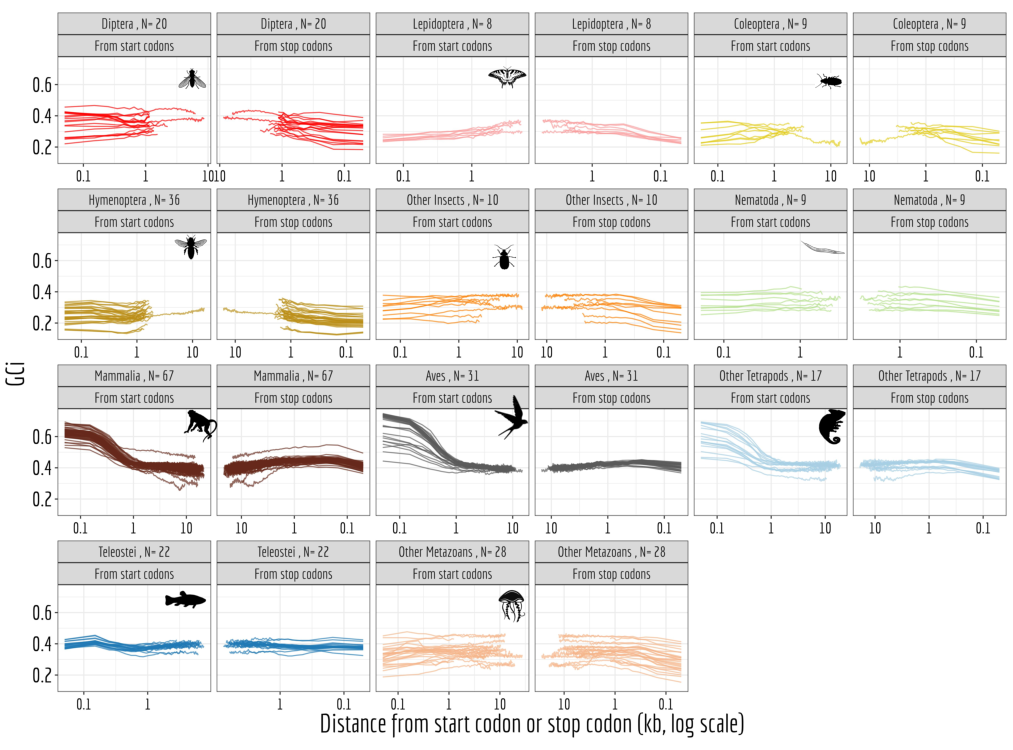
\includegraphics[width=\textwidth] {Figure7_supp.pdf}
    \end{center}                                                                       
    \caption[Correlations between gene expression levels and AS rates differ among species]{\textbf{Correlations between gene expression levels and AS rates differ among species.} \textbf{A,B}: Relationship between the average AS rate of major-isoform introns (with $\mathrm{N_s+N_a}\geq100$, see \hyperref[fig:AS2]{Fig. 2}) and the expression levels of the corresponding genes (FPKM, log scale). We divided major-isoform introns into 5\% bins according to the expression level of the corresponding genes and computed for each bin the average AS rate and the median expression level. Error bars represent the standard error of the mean. \textbf{A}: \textit{Homo sapiens}, \textbf{B}: \textit{Drosophila melanogaster}. This analysis was performed on all protein-coding genes (\textit{blue}) and BUSCO genes (\textit{light blue}). Pearson correlation presented here was computed on protein-coding genes.}
    \label{supp_fig:AS7}
\end{figure}


\begin{figure}[t]   
    \begin{center}                                                                       
        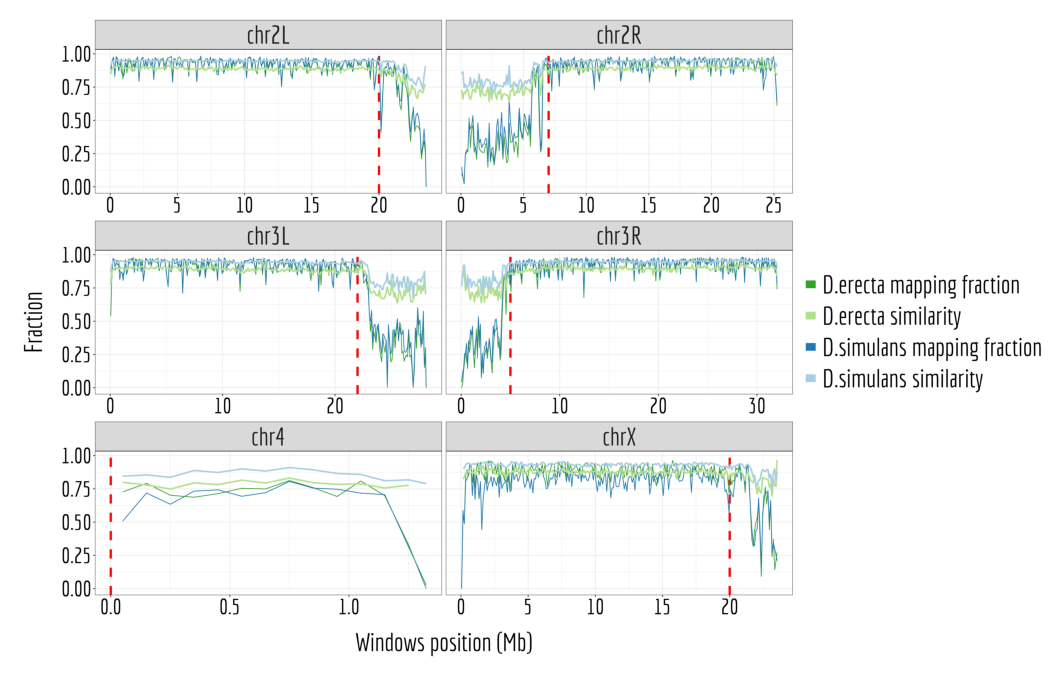
\includegraphics[width=\textwidth] {Figure8_supp.pdf}
    \end{center}                                                                       
    \caption[Relationship between AS rates and \textit{N}$_{\text{e}}$ proxies, for all major-isoform introns, low-AS major-isoform introns (\textit{i.e.} major-isoform introns that do not have any abundant spliced variants) and high-AS major-isoform introns (\textit{i.e.} major-isoform introns having at least one abundant spliced variants).]{\textbf{Relationship between AS rates and \textit{N}$_{\text{e}}$ proxies, for all major-isoform introns, low-AS major-isoform introns (\textit{i.e.} major-isoform introns that do not have any abundant spliced variants) and high-AS major-isoform introns (\textit{i.e.} major-isoform introns having at least one abundant spliced variants).} Relationship between the average AS rate of all major-isoform introns (\textbf{A,B,C}) or low-AS major-isoform introns (\textbf{D,E,F}) or high-AS major-isoform introns (\textbf{G,H,I}) and longevity (days, log scale) (\textbf{A,D,G}) or body length (cm, log scale) (\textbf{B,E,H}) or the ${dN}/{dS}$ ratio (\textbf{C,F,I}).} 
    \label{supp_fig:AS8}
\end{figure}

\begin{figure}[t]   
    \begin{center}                                                                       
        \includegraphics[width=\textwidth] {Figure9_supp.pdf}
    \end{center}                                                                       
    \caption[Relationship between the proportion of frame-preserving SVs and \textit{N}$_{\text{e}}$ proxies]{\textbf{Relationship between the proportion of frame-preserving SVs and \textit{N}$_{\text{e}}$ proxies.} \textbf{A,B}: Relationship between the proportion of frame-preserving SVs among abundant SVs, and the body length (cm, log scale) of the organism (\textbf{A}) or the ${dN}/{dS}$ ratio (\textbf{B}). Each dot represents one species. All protein-coding genes were used in the analysis.}
    \label{supp_fig:AS9}
\end{figure}


\begin{figure}[t]   
    \begin{center}                                                                       
        \includegraphics[width=\textwidth] {Figure10_supp.pdf}
    \end{center}                                                                       
    \caption[The \textit{per}-gene AS rate is negatively correlated with \textit{N}$_{\text{e}}$]{\textbf{The \textit{per}-gene AS rate is negatively correlated with \textit{N}$_{\text{e}}$.} Relationship between \textit{per}-gene average AS rates and \textit{N}$_{\text{e}}$ proxies. We use as inverse \textit{N}$_{\text{e}}$ proxies the longevity (days, log scale) (\textbf{A,D}) or the body length (cm, log scale) (\textbf{B,E}) or the ${dN}/{dS}$ ratio (\textbf{C,F}). The analysis was done on BUSCO genes (\textbf{A,B,C}) and on all protein-coding genes (\textbf{D,E,F}).}
    \label{supp_fig:AS10}
\end{figure}

\begin{figure}[t]   
    \begin{center}                                                                       
        \includegraphics[width=\textwidth] {Figure11_supp.pdf}
    \end{center}                                                                       
    \caption[Description of the bioinformatic analyses pipeline]{\textbf{Description of the bioinformatic analyses pipeline.} First, we retrieved genomic sequences and annotations from the NCBI Genomes database. We aligned RNA-seq reads with HISAT2 on the corresponding reference genomes, to analyze various variables (see \hyperref[fig:AS2]{Fig. 2}), to compute the AS rate, and to estimate gene expression using Cufflinks. To compute ${dN}/{dS}$, we first identified BUSCO genes with BUSCOv3 and aligned their coding sequences (CDS) using PRANK (codon model). We reconstructed a phylogenetic tree using RAxML-NG with 461 multiple alignments. Using bio++, we estimated ${dN}/{dS}$ along the phylogenetic tree on concatenated alignments.} 
    \label{supp_fig:AS11}
\end{figure}
